\documentclass[11pt,a4paper]{book}
\usepackage[utf8]{inputenc}
\usepackage{siunitx}
\usepackage[siunitx]{circuitikz}
\usepackage[english]{babel}
\usepackage{amsmath}
\usepackage{amsfonts}
\usepackage{amssymb}
\usepackage{caption}
\usepackage{subcaption}
\usepackage{pgfplots}
\usepackage{graphicx}
\author{Ege Özkan}
\title{CENG 215 \\ \large{Circuits and Electronics Lecture Notes}}
\begin{document}
\newcommand{\vin}{\ensuremath{V_\text{in}}}
\newcommand{\vout}{\ensuremath{V_\text{out}}}
\newcommand{\diffd}{\ensuremath{\text{d}}}
\newcommand{\diff}[2]{\ensuremath{\frac{\diffd}{\diffd #1} \left( #2 \right)}}
\newcommand{\sdif}[2]{\ensuremath{\frac{\diffd #1}{\diffd #2}}}

\maketitle

\chapter{Introduction - October 15, 2020}


\section{Abstractions}

Recall the Newton's formula $F=ma$, which defines the relationship between force, mass and acceleration. This formula modals acceleration using force and mass. However, according to this model, there is no connection between mass and speed. Consider now, the Einstein's equation:

\begin{equation}
m = \frac{m_0}{\sqrt{1 - \frac{v^2}{c^2}}}
\end{equation}

As this equation shows, speed affects mass. The abstractions ignore certain connections for the sake of simplicity. Likewise, electrical engineering, based on Maxwell's Equations, create abstractions, notably, this lecture deals with the \textit{Lumped Circuit Abstraction}.

Consider a statement in a high level programming language \texttt{int n = 3;}, this basic statment goes through many abstractions eventually reaching circuitery.

\section{Circuits}

\begin{figure}[httb]
\begin{circuitikz} \draw
(0,0) to [V] ++ (2, 0) -- (2,2) to [R] (0, 2) -- (0, 0)
;
\end{circuitikz}
\caption{A simple cirucit abstraction}
\end{figure}


From this abstraction, arises the \textbf{Ohm's Law}

\begin{equation}
v = iR
\end{equation}


\subsection{Two Terminal Element}

\begin{center}
\begin{circuitikz}[american voltages]
\draw
  (0,0) to [short, *-,i_ = $i$] (2,0) 
  to [generic] (2,2) -- (0,2)
  (0, 0)to [open, v^>=$v$, *-] (0,2)
  to [short, *-] (0,2)
;
\end{circuitikz}
\end{center}

Two terminal elements include batteries, resistors, capacitors, etc...

\subsubsection{Battery}

Batteries provide voltage and can be bind into serial or paralel.

\begin{center}
\begin{circuitikz}[american voltages]
\draw
  (0,0) to [short, *-] (2,0)
  to [V, l_=$v$] (2,2) -- (0,2)
  to [short, *-] (0,2)
;
\end{circuitikz}
\end{center}

Below are power (in watts) and energy (in Jouless or watt-seconds) for batteries.

\begin{equation}
P = vi
\label{Power in watt}
\end{equation}

\begin{equation}
w = Pt
\label{Energy formula in joules or watt-seconds}
\end{equation}

Enery formula can also be represented as:

\begin{equation}
w = \int_{t_1}^{t_2} v(t) i(t) \text{d}t
\end{equation}

\subsubsection{Resistance}

\begin{center}
\begin{circuitikz}[american voltages]
\draw
  (0,0) to [short, *-, i_=$i$] (1,0)
  to [tline, l_=$R$] (3,0) to [short, -*] (4,0)
;
\end{circuitikz}
\end{center}

Imagine a generic tube with length $l$, resistivity $\rho$ and cross sectional area $a$, in this case, the Resistance of the element $R$ is

\begin{equation}
R = \rho \frac{l}{a}
\end{equation}

The resistance can be showed as:

\begin{center}
\begin{circuitikz}[american voltages]
\draw
  (0,0) to [short, *-, i_=$i$] (1,0)
  to [R, l_=\text{$R$, $V$}] (3,0) to [short, -*] (4,0)
;
\end{circuitikz}
\end{center}

Where the Ohm's Law state:

\begin{equation}
v = Ri
\end{equation}

or alternativelly

\begin{equation}
i = Gv
\end{equation}

Where $G$ is conductance, whose SI unit is siemens and defined as $\frac{1}{R}$

\subsubsection{Ideal Voltage Source}

Ideal Voltage source can be represnted by:

\begin{center}
\begin{circuitikz}[american voltages]
\draw
  (0,0) to [short, *-] (1,0)
  to [battery1, v<=$v(t)$, i_=$i$] (3,0) to [short, -*] (4,0)
;
\end{circuitikz}
\end{center}

\begin{center}
\begin{circuitikz}[american voltages]
\draw
  (0,0) to [short, *-] (1,0)
  to [V, v<=$v(t)$, i_=$i$] (3,0) to [short, -*] (4,0)
;
\end{circuitikz}
\end{center}

In general, any voltage soucre can be drawn as

\begin{center}
\begin{circuitikz}[american voltages]
\draw
  (0,0) to [short, *-] (2,0)
  to [R, l_ = $r$] (2,2)
  to [V, l_=$v$, i_=$i$] (0,2) 
  to [short, *-] (0,2)
;
\end{circuitikz}
\end{center}

Where $r$ is the internal resistence that arise from the material itself. An ideal voltage source would be able to provide the same current no matter what the voltage is, however this is not possible in real life, where any voltage source has a $r$

\chapter{Resistive Networks - 22 October, 2020}
\begin{figure}[h]
\begin{circuitikz}[american voltages]
\draw (0,2)
	to [short, *-] (-2 , 2)
	to [V, v=10<\volt>, i_=0<\ampere>] (-2,0)
	to [short, -*] (0, 0);
\draw (4, 2)
	to [short, *-] (2, 2)
	to [V, v=10<\volt>, i_=0<\ampere>] (2,0)
	to [short, -*] (4, 0)
	to [R, l_={$\infty$}] (4, 2);
\end{circuitikz}\\
\begin{circuitikz}[american voltages]
\draw (0,2)
	to [short] (-2 , 2)
	to [V, v=10<\volt>, i_=$\infty$] (-2,0)
	to [short] (0, 0)
	to [short] (0, 2);
\draw (4, 2)
	to [short] (2, 2)
	to [V, v=10<\volt>, i_=$\infty$] (2,0)
	to [short] (4, 0)
	to [R, l_={0<\ohm>}] (4, 2);
\end{circuitikz}
\caption{An open circuit is equivalent to a circuit with a resistor with an infinite resistance. Whereas a short cirucit can be modelled as a circuit with zero resistence.}
\end{figure}

The perfect current source is a current source that can supply current in any voltage.


\section{Signals}
\begin{figure}[h]
\begin{subfigure}[b]{\textwidth}
\centering
\begin{tikzpicture}
\begin{axis}
\addplot[domain=0:10, samples=100, color=red]{sin(deg(x))};
\end{axis}
\end{tikzpicture}
\end{subfigure}

\begin{subfigure}[b]{\textwidth}
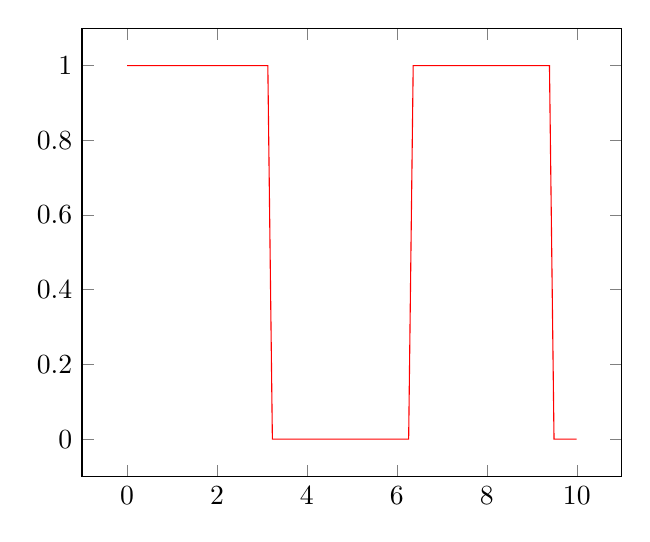
\begin{tikzpicture}
\begin{axis}
\addplot[domain=0:10, samples=100, color=red]{floor(sin(deg(x))) + 1};
\end{axis}
\end{tikzpicture}
\end{subfigure}
\caption{Two signals.}
\label{fig:signals}
\end{figure}

Signals can be analog or digital. In Figure \ref{fig:signals}, the sinosodial signals, which has continous values is an analog signal. Where it is represented via the $v(t) = A\sin(\omega t + \phi)$, where $A$ is its amplitude, $\omega$ is its frequency and $\phi$ is its phase, it is analog because it has \textit{continous} values. In the meantime, the second signal is a digital signal as it has \textit{discrete} and quantised values.\\

Digital signals trade precision about the signal with \textit{immunity towards the noise}.

\begin{description}
\item[Resistance] A measure of the ability of the device to consume energy.
\item[Capacitence] A measure of the ability of the device to store energy in the form of potential energy. (voltage).
\item[Inductance] A measure of the ability of the device to store energy as the moving charge (current).
\end{description}

\section{Resistive Networks}

\begin{center}
\begin{circuitikz}[american voltages]
\draw (2,0)
	to [short] (-2, 0);
\draw (-2, 3)
	to [V^>=$V$] (-2, 0);
\draw (-2, 3)
	to [R=$R_1$, v=$v_1$, i=$i_1$] (2, 3)
	to [R=$R_2$, v=$v_2$, i=$i_2$] (2, 0);
\draw (2, 3)
	to [R=$R_3$, v=$v_3$, i=$i_3$](6, 3)
	to [R=$R_4$, v=$v_4$, i=$i_4$](6, 0)
	to [short] (2, 0);
\end{circuitikz}
\end{center}
This sort of circuits can be analysed using two laws, \textbf{Kirchoff's Current Law} (KCL) and \textbf{Kirchoff's Voltage Law} (KVL).

\subsection{Kirchoff's Current Law}

\begin{center}
\begin{circuitikz}[american voltages]
\draw (2,2)
	to [short, i_=$i_1$] (0,0);
\draw(2, 0)
	to [short, -*, i_=$i_2$] (0, 0);
\draw(2, -2)
	to [short, i_ =$i_3$] (0,0);
\draw(-2, 2)
	to [short, i_=$i_4$](0,0);
\draw(-2, 0)
	to [short, -*, i_=$i_5$] (0, 0);
\draw(-2, -2)
	to [short, i_ =$i_6$] (0,0);
\end{circuitikz}
\end{center}
Kirchoff's current law state that the sum of currents entering a node must equal zero.\\

\begin{equation}
\sum_{n = 1}^6 i_n = 0
\end{equation}

When one takes the directions of the currents into account, this means that the \textit{currents entering a node must equal the curents exiting a node}.

\subsection{Kirchoff's Voltage Law}

\begin{center}
\begin{circuitikz}[american voltages]
\draw (2,0)
	to [short] (-2, 0);
\draw (-2, 3)
	to [V^>=$V_1$] (-2, 0);
\draw (-2, 3)
	to [R=$R_1$, v=$v_1$, i=$i_1$] (2, 3)
	to [R=$R_2$, v=$v_2$, i=$i_2$] (2, 0);
\draw (6, 3)
	to [R=$R_3$, v=$v_3$, i_=$i_3$](2, 3);
\draw(6,3)
	to [V=$V_2$](6, 0)
	to [short] (2, 0);
\end{circuitikz}
\end{center}

Consider three loops, if clockwise, starting from the battery's top, each node is called a, b, c, d then for loop abcda:

\begin{align*}
v_{ba} + v_{bc} + v_{cd} + v_{da} = 0\\
v_{ab} = v_1 = R_1 i_1\\
v_{bc} = v_3 = -R_3 i_3 \\
v_{cd} = V_2\\
v_{da} = -V_1\\
V_2 - V_1 + R_1i_1 -R_3i_3 = 0
\end{align*}

In general, KVL states that, for a closed loop $L$:

\begin{equation}
\sum^{L} v_{L_i} = 0
\end{equation}

That is, sum of voltages in a  closed loop equals to zero.

\subsection{Node Voltage Method}
\begin{center}
\begin{circuitikz}[american voltages]
\draw (2,0)
	to [short] (-2, 0);
\draw (-2, 3)
	to [V^>=32<\volt>] (-2, 0);
\draw (-2, 3)
	to [R=2<\ohm>, i=$i_1$] (2, 3)
	to [R=8<\ohm>, i=$i_3$] (2, 0);
\draw (6, 3)
	to [R=4<\ohm>, i_=$i_2$](2, 3);
\draw(6,3)
	to [V=20<\volt>](6, 0)
	to [short] (2, 0)
	node[ground]{};
\end{circuitikz}
\end{center}

By denoting voltages at nodes as $v_a$, $v_b$, $v_c$ and $v_d$ and connect $v_d$ at the ground, making it effectively zero.\\

\begin{align}
i_1 + i_2 - i_3 = 0 & (\text{  KCL at node b.})\\
i_1 = \frac{v_a - v_b}{2} = \frac{32 - v_b}{2}\\
i_2 = \frac{v_c - v_b}{4} = \frac{20 - v_b}{4}\\
i_3 = \frac{v_b - 0}{8} = \frac{v_b}{8}\\
\end{align}

And therefore subsituting values of $i_1, i_2$ and $i_3$ at Equation 2.3\\

\begin{align*}
\frac{32 - v_b}{2} + \frac{20 - v_b}{4} - \frac{v_b}{8} = 0\\
128 - 4v_b + 40 - 2v_b - v_b = 0\\
v_b = 24\text{V}
\end{align*}

And from here, one can calculate the currents.

\begin{align*}
i_1 = \frac{32 - 24}{2} = \text{ 4A}\\
i_2 = \frac{20 - 24}{4} = \text{ 1A}\\
i_3 = \text{ 3A}\\
\end{align*}

\begin{circuitikz}
\draw (0,0)
	to [battery, v^>=5<\volt>] (0, 6)
	to [short] (4, 6)
	to [R=1<\kilo\ohm>] (4, 4)
	to [R=1<\kilo\ohm>] (4, 2)
	to [R=1<\kilo\ohm>] (4, 0)
	to [short] (0, 0);
\end{circuitikz}

\chapter{Resistive Networks (Cont`d) - November 12, 2020}

\section{Voltage Divider}
\begin{circuitikz}[american voltages]
\draw (0,4)
	to [short, i_=$i$] (2.5, 4)
	to [R = $R_1$] (2.5, 2)
	to [R = $R_2$] (2.5, 0);
\draw (0,4)
	to [V, v=$\vin$] (0, 0)
	to [short] (2.5, 0)
	to [short, -o] (4, 0);
\draw (2.5, 2)
	to [short, -o] (4, 2)
	to [open, v=$\vout$] (4, 0);
\end{circuitikz}

The above circuit is refeered to as a Voltage divider cricuit, taking into account that $\vout$ is the voltage accross the $R_2$ resister, using the Ohm's law, we can find:

\begin{align*}
i &= \frac{\vin}{R_1 + R_2}\\
\vout &= i R_2\\
\vout &= R_2 \frac{\vin}{R_1 + R_2}
\end{align*}

And hence:

\begin{equation}
\vout = \vin \frac{R_2}{R_1 + R_2}
\end{equation}


\chapter{Energy Storage Elements - November 12, 2020}

Capacitive and Inductive effects are used to store energy.

\section{Capacitor}

Consisting of  two plates, seperated by an insulator, whose dielectric permitivity is $\varepsilon$, the area of the plates is $A$, and the distance between them is $l$, when a voltage source is applied on these plates, positive charge $q$ will accumulate on the one side, and the negative on the other side creating an electrical field $E$, where $v$ is the voltage between them.\\

\begin{align*}
E(t) &= \frac{q(t)}{\varepsilon A(t)}\\
v(t) &= l(t) \times E(t)
\end{align*}

Therefore

\begin{align*}
q(t) = \frac{\varepsilon A(t)}{l(t)} v(t)
\end{align*}

Here, we say that:

\begin{align*}
C(t) = \frac{\varepsilon A(t)}{l(t)}
\end{align*}

Therefore, unifying these formulas

\begin{equation}
q(t) = C(t) \times v(t)
\end{equation}

Where $C$ is the capacitance, whose value is Coulombs/Volt or Farad (F). Capacitor exibits proportional relation between voltage and stored charge. since rate of charge transfer is current, that is $\sdif{q(t)}{t} = i(t)$ We can say that

\begin{equation}
i(t) = C \diff{t}{v(t)}
\end{equation}

And likewise, from the same relation:

\begin{equation}
v(t) = \frac{1}{C} \int_{-\infty}^{t} i(t) \diffd t
\end{equation}

When $n$ capacitors are connected in series, their equivalent capacitance is:

\begin{equation}
\frac{1}{C_{\text{eq}}} = \sum_{i = 1}^{n} \frac{1}{C_i}
\end{equation}

When $n$ capacitors are connected in parallel, their equivalent capacitance is:

\begin{equation}
C_{\text{eq}} = \sum_{i = 1}^n C_i
\end{equation}

\section{Inductor}

Inductor is a wire wrapped around a ring of crossectional area $A$, and with magnetic permatibility $\mu$ of circumferance $l$, wrapped around $N$ times, and a current $i$ is applied, a magnatic flux $\Phi$ of density $B$ is generated. This magnetic field can then be used to store energy, similar to how a capacitor uses electric field to store energy.\\

\begin{align*}
B(t) &= \frac{\mu N i(t)}{l(t)}\\
\Phi(t) &= A(t) \times B(t)
\lambda(t) = N \Phi(t) = \frac{\mu N^2 A(t)}{l(t)} i(t)
\end{align*}

Where, $\lambda$ is the total flux.

The Inductance ($L$) is generated, it is defined as the ratio of fthe voltage to the rate of change of the current. Furthermore, $L(t)$ is said to be

\begin{equation}
L(t) = \frac{\mu N^2 A(t)}{l(t)}
\end{equation}

And hence

\begin{equation}
\lambda(t) = L(t) i(t)
\end{equation}

Also, voltage and current of the inductor is defined as:

\begin{align}
v(t) &= L \sdif{i(t)}{t}\\
i(t) &= \frac{1}{L} \int_{- \infty}^{t} v(t) \diffd t
\end{align}

Inductance has the unit Henry, (H) is the SI unit system, their equivalence follows the rules of the resistence.

\section{Summary}

\subsubsection{Capacitor}

\begin{circuitikz}[american voltages]
\draw (0,0)
	to [short, i_=$i$, *-] (1, 0)
	to [C={$C$}] (3.5, 0)
	to [short, -*] (4, 0);
\draw (0, -1)
	to [open, v=$v$] (4, -1);
\end{circuitikz}

\begin{equation}
i(t) = C \sdif{v(t)}{t}
\end{equation}

If a voltage source is connected to a capacitor without nothing else, the current and capacitance will be zero.

\subsubsection{Inductor}

\begin{circuitikz}[american voltages]
\draw (0,0)
	to [short, i_=$i$,  *-] (1, 0)
	to [L={$L$}] (3.5, 0)
	to [short, -*] (4, 0);
\draw (0, -1)
	to [open, v=$v$] (4, -1);
\end{circuitikz}

\begin{equation}
v(t) = L \sdif{i(t)}{t}
\end{equation}

If a current source is connected to a inductor without nothing else, the current and inductance will be zero.

\chapter{Network Theorems - November 13, 2020}

\begin{circuitikz}[american]
\draw (0,0)
	to [V=1<\volt>] (0, -3)
	to [short] (3, -3)
	to [R=4<\ohm>] (3, 0)
	to [R=1<\ohm>, *-] (0, 0);
\draw (3, -3)
	to [short] (6, -3)
	to [R=5<\ohm>, -*] (6, 0);
\draw(3, 0)
	to [I=2<\ampere>] (6, 0);
\draw(6, -3)
	to [short] (9, -3)
	to [I=1<\ampere>](9, 0)
	to [short] (6, 0);
\draw (3, 0)
	to [short] (3.5, 1)
	to [R=2<\ohm>] (5.5, 1)
	to [short] (6, 0);
\node[draw] at (2.6, 0.5) {1};
\node[draw] at (6.4, 0.5) {2};
\node[ground] at (4.5, -3) {};
\end{circuitikz}

Here, after grounding at the bottom, hence giving it zero volts voltage, we can perform KVL at Nodes 1 and 2.

\begin{align*}
\frac{V_1 - 1}{1} + \frac{V_1}{4} + \frac{V_1 - V_2}{2} + 2 = 0\\
-2 + \frac{V_2}{5} + \frac{V_2-V_1}{2} - 1 = 0\\
V_1 = 0.65\text{V}\\
V_2 = 4.75\text{V}\\
i = 0.95 \text{A}
\end{align*}

The current formulas above arise from the node-voltage method being performed at both nodes.
\subsubsection{Resistive Adder}

\begin{circuitikz}[american]
\draw (0,0)
	to [R=$R$] (0, -2)
	to [V=$v_1$] (0, -4);
\draw (2,0)
	to [R=$R$] (2, -2)
	to [V=$v_2$] (2, -4);
\draw (4,0)
	to [R=$R$] (4, -2)
	to [V=$v_3$] (4, -4);
\draw (6,0)
	to [R=$R$] (6, -2)
	to [V=$v_4$] (6, -4);
\draw (0, 0)
	to [short, -*](8, 0)
	to [open, v=$v_0$] (8, -4)
	to [short, *-] (0,-4);
\end{circuitikz}

Where we can conclude, ısing the node voltage method:

\begin{equation}
\frac{v_0 - v_1}{R} + \frac{v_0 - v_2}{R} + \frac{v_0 - v_3}{R} + \frac{v_0 - v_4}{R}
\end{equation}

\begin{equation}
v_0 = \frac{1}{4} \left( v_1 + v_2 + v_3 + v_4 \right)
\end{equation}

\subsubsection{Dependant Sources}

Dependant sources are sources whose values depend on the values of other points. There are dependant voltage sources and dependant current sources.\\

\begin{circuitikz}[american]
\draw (3,0)
	to [short, *-] (0, 0)
	to [R=1<\kilo\ohm>] (0, -2)
	to [V=1<\volt>] (0, -4)
	to [short] (6, -4)
	to [cI=$\frac{1}{100\si{\ohm}}v$] (6, 0)
	to [short, -*] (9, 0)
	to [R=1<\kilo\ohm>](9,-4)
	to [short] (6, -4);
\draw(3, 0)
	to [R=1<\kilo\ohm>] (3, -2)
	to [V=2<\volt>] (3, -4);
\node[circ] at (3,0) {$v$};
\node[circ] at (9,0) {$v_0=?$};
\end{circuitikz}

Here we start by calculating $v$, the current of the dependant current source depends on this value.

\begin{align*}
v &= \frac{1}{2} (1 + 2) = 1.5\si{\volt}\\
v_0 &= I. 1\si{\kilo\ohm}\\
&= \frac{1}{100} \times 1.5 \times 1 \si{\kilo\ohm}\\
&= 15 \si{\volt}
\end{align*}

\section{Thevenin Network Theorems}

If the system is linear, any network can be represented by a sinlge voltage source and a resistor.\\

\begin{circuitikz}[american]
\draw (0,0) 
	to [R=$R_T$, o-] (-3, 0)
	to [V=$V_T$] (-3, -3)
	to [short, -o] (0, -3);
\end{circuitikz}


\subsubsection{Example}

Given an example circuit of the form:

\begin{circuitikz}[american]
\draw (0,0)
	to [short] (3, 0) 
	to [R=2<\ohm>] (3, 3)
	to [R=1<\ohm>] (0, 3)
	to [V=3<\volt>] (0, 0);
\draw (3, 0) to [short, -*] (4, 0);
\draw (3, 3) to [short, -*] (4, 3)
	to [open, v=$V_R$] (4, 0);
\end{circuitikz}

Where $V_R$ is taken the thevenin voltage, $V_T$. To calculate $V_R$, a simple KVL would do, where $i$ the main current of the circuit $i = 1 \si{\ampere}$ and hence, $V_R = 1 \si{\ampere}\times 2 \si{\ohm} = 2 \si{\volt}$ and hence, $V_T = 2 \si{\volt}$.\\

Then, short-circuit between the output terminals, and calculate the $i$ again, the resistor will be short circuited, with $i_2 = 3\si{\ampere}$ And hence, we can now calculate the $R_T$ by saying that the current in the thevenin equivalent circuit will equal $i_2$. Calculating this, yields $R_T = \frac{2}{3} \si{\ohm}$. And hence, the thevenin equivalent circuit is:

\begin{circuitikz}[american]
\draw (0,0) 
	to [R=$\frac{2}{3}\si{\ohm}$, o-] (-3, 0)
	to [V=2<\volt>] (-3, -3)
	to [short, -o] (0, -3);
\end{circuitikz}

\subsubsection{Example}
\begin{circuitikz}[american]
\draw (0,0)
	to [short] (3, 0) 
	to [R=2<\ohm>] (3, 3)
	to [R=2<\ohm>] (0, 3);
\draw(0,0)
	to [I=2<\ampere>] (0, 3);
\draw (3, 0) to [short, -*] (4, 0);
\draw (3, 3) to [short, -*] (4, 3)
	to [open, v=$V_R$] (4, 0);
\end{circuitikz}

Start by finding the voltage accross the resistor once more, which is $V_R = 2 \si{\ohm} \times 2 \si{\ampere} = 4 \si{\volt}$ Hence, so is $V_T$, shortcircuiting the resistor once more, since this is a current source, $i$ is still the same (2A) and can be used to calculate $R_T$ again, which is $R_T = 2 \si{\ohm}$\\

\begin{circuitikz}[american]
\draw (0,0) 
	to [R=$2\si{\ohm}$, a=$R_T$, o-] (-3, 0)
	to [V=4<\volt>, a=$V_T$] (-3, -3)
	to [short, -o] (0, -3);
\end{circuitikz}

\subsubsection{Example}
\begin{circuitikz}[american]
\draw (0,0)
	to [short] (3.5,0) 
	to [R=1<\kilo\ohm>, -*] (3.5, 3)
	to [short] (0, 3)
	to [V=$2\cos(\omega t)$] (0, 0);
\draw(3.5, 0)
	to [short] (9, 0)
	to [R=2<\kilo\ohm>] (9, 3)
	to [short] (6, 3)
	to [cI=$\frac{8}{100\si{\ohm}} v_i$] (6, 0);
\draw (9, 0) to [short, -o] (10, 0);
\draw (9, 3) to [short, -o] (10, 3)
	to [open, v=$V_o$](10,0);
\node[circ] at (3.5, 3) {$V_i$};
\end{circuitikz}

Here, to calculate $V_o$, we first need to calculate $V_i$, $V_i$ is of course equivalent to the voltage source at the left side, and hence $V_i = 2 \cos(\omega t)$ and hence the current at the left hand side, $I = - \frac{8}{100} 2 \cos (\omega t) \times 2000$, and hence, $V_o = -320 \cos(\omega t)$.\\

To find the equivalent resistor, we short cirucit the open ports, and once again find the current, which equals to the current source, and then, we must use the resulting current in the equivalent circuit to determine the resistance, which is $R_T = 2 \si{\kilo\ohm}$.\\

\begin{circuitikz}[american]
\draw (0,0) 
	to [R=2<\kilo\ohm>, a=$R_T$, o-] (-3, 0)
	to [V=$-320 \cos(\omega t)$, a=$V_T$] (-3, -3)
	to [short, -o] (0, -3);
\end{circuitikz}

\section{Norton Theorem}

Norton theorem states that any linear circuit can be represented using a single current source, and a resistance.\\

\begin{circuitikz}[american]
\draw (0,0) 
	to [short, *-] (-4, 0)
	to [I=$I_n$] (-4, 3)
	to [short, -*] (0, 3);
\draw (-2, 0)
	to [R=$R_N$] (-2, 3);
\end{circuitikz}




\end{document}